\documentclass[border=4pt,12pt]{standalone}
% House style for redrawn exam diagrams (diagram-v4: 0.4pt lines, filled -latex arrows, fine dashes; stipple and hatching drawn as real dots/lines (no PDF/SVG patterns, so they render in every browser and at any scale); transparent background). Every figure \input's this.
\usepackage{amsmath,amssymb}
\usepackage{txfonts}
\usepackage{pdfrender,xcolor}
% \halo{text}: label on shading. The shading stops just around each letter's outline (a thin knock-out that follows the
% glyphs, like the papers' typesetting), never a box. Owner: "I don't want a box around the text".
\newcommand{\halo}[1]{\leavevmode\rlap{\pdfrender{TextRenderingMode=2,LineWidth=2.2pt,LineJoinStyle=1,StrokeColor=white,FillColor=white}#1}#1}
\usepackage{tikz,pgfplots}
\pgfplotsset{compat=1.18}
\usetikzlibrary{arrows.meta,calc,angles,quotes,patterns,patterns.meta,intersections,positioning,decorations.markings,shapes.geometric}
% Stipple and hatching are drawn as actual dots / lines clipped to the region (path picture), NOT as pattern fills:
% SVG <pattern> fills vanish or blur when browsers scale the image, so the owner could not see the shading.
% Each dot is a 0.72pt square (keeps SVGs small; reads as a dot at print size). Dots sit on one global staggered grid, so neighbouring regions line up.
\makeatletter
\newdimen\ex@x \newdimen\ex@y \newdimen\ex@xa \newdimen\ex@ya \newdimen\ex@xb \newdimen\ex@yb \newcount\ex@row
\def\exam@stipplecolor{black!75}\def\exam@dotr{0.42pt}\def\exam@dotgap{2.5}
\def\ex@rowdots{\ifdim\ex@x<\ex@xb \pgfpathrectangle{\pgfqpoint{\dimexpr\ex@x-0.36pt\relax}{\dimexpr\ex@y-0.36pt\relax}}{\pgfqpoint{0.72pt}{0.72pt}}\advance\ex@x by \exam@dotgap pt\relax\expandafter\ex@rowdots\fi}
\def\exam@stipple{%
  \pgftransformreset% dots are sized in real points even inside scaled pictures
  \pgfpointanchor{path picture bounding box}{south west}\ex@xa=\pgf@x \ex@ya=\pgf@y
  \pgfpointanchor{path picture bounding box}{north east}\ex@xb=\pgf@x \ex@yb=\pgf@y
  \pgfsetfillcolor{\exam@stipplecolor}\pgfmathsetmacro\ex@h{\exam@dotgap/2}%
  \pgfmathtruncatemacro\ex@r{floor(\ex@ya/\ex@h)-1}\ex@row=\ex@r\relax
  \ex@y=\ex@r\dimexpr\ex@h pt\relax
  \loop\ifdim\ex@y<\ex@yb
    \pgfmathtruncatemacro\ex@c{floor(\ex@xa/\exam@dotgap)-1}\ex@x=\ex@c\dimexpr\exam@dotgap pt\relax
    \ifodd\ex@row \advance\ex@x by \ex@h pt\fi
    \ex@rowdots
    \advance\ex@y by \ex@h pt \advance\ex@row by 1
    \ifnum\numexpr\ex@row-(\ex@row/4)*4\relax=0 \pgfusepath{fill}\fi% flush every 4 rows: bounded TeX memory, few clip copies in the SVG
  \repeat\pgfusepath{fill}}
\newdimen\ex@d
\def\exam@hatch#1{% #1 = 1 for /, -1 for \ ; lines 45 degrees, 3pt apart
  \pgftransformreset
  \pgfpointanchor{path picture bounding box}{south west}\ex@xa=\pgf@x \ex@ya=\pgf@y
  \pgfpointanchor{path picture bounding box}{north east}\ex@xb=\pgf@x \ex@yb=\pgf@y
  \ex@d=\dimexpr\ex@yb-\ex@ya\relax \ex@x=\dimexpr\ex@xa-\ex@d\relax
  \loop\ifdim\ex@x<\ex@xb
    \ifnum#1>0 \pgfpathmoveto{\pgfqpoint{\ex@x}{\ex@ya}}\pgfpathlineto{\pgfqpoint{\dimexpr\ex@x+\ex@d\relax}{\ex@yb}}%
    \else \pgfpathmoveto{\pgfqpoint{\ex@x}{\ex@yb}}\pgfpathlineto{\pgfqpoint{\dimexpr\ex@x+\ex@d\relax}{\ex@ya}}\fi
    \advance\ex@x by 4.24pt
  \repeat
  \pgfsetlinewidth{0.4pt}\pgfsetstrokecolor{black}\pgfusepath{stroke}}
\def\examstipple{\exam@stipple}\def\examhatch{\exam@hatch}\def\examsetstipplecolor#1{\def\exam@stipplecolor{#1}}\def\examsetdotgap#1{\def\exam@dotgap{#1}}
\makeatother
% (legacy pattern kept for old files)
% staggered stipple like the NESA papers' dotted shading
\pgfdeclarepatternformonly{exam stipple}{\pgfpointorigin}{\pgfqpoint{2.2pt}{2.2pt}}{\pgfqpoint{2.2pt}{2.2pt}}{%
  \pgfpathcircle{\pgfqpoint{0.55pt}{0.55pt}}{0.42pt}\pgfpathcircle{\pgfqpoint{1.65pt}{1.65pt}}{0.42pt}\pgfusepath{fill}}
\tikzset{
  every picture/.style={line width=0.6pt, >={Latex[length=2mm,width=1.3mm]}},
  curve/.style={line width=0.6pt},
  open arrow/.style={-{Latex[length=2mm,width=1.3mm]}},  % owner: filled -latex heads everywhere, no open chevrons
  aux/.style={dash pattern=on 2pt off 1.5pt, line width=0.6pt},
  shade/.code={\def\exA{#1}\def\exB{none}\ifx\exA\exB\else\pgfkeysalso{fill=black!18}\fi},
  shade/.default=on,
  shade dots/.style={fill=none, path picture={\examstipple}},
  stipple color/.code={\examsetstipplecolor{#1}},
  stipple gap/.code={\examsetdotgap{#1}},
  shade dense dots/.style={fill=none, stipple gap=1.6, path picture={\examstipple}},
  shade hatch/.style={fill=none, path picture={\examhatch{1}}},
  shade hatch reverse/.style={fill=none, path picture={\examhatch{-1}}},
  shade solid/.style={fill=black},
  pt/.style={circle, fill, inner sep=1.1pt},
  open pt/.style={circle, draw, fill=white, inner sep=1.1pt},
}
\pgfplotsset{
  exam axes/.style={axis lines=middle, axis line style={->}, xlabel={$x$}, ylabel={$y$},
    xlabel style={anchor=west}, ylabel style={anchor=south}, tick label style={font=\small},
    every axis plot/.append style={line width=0.6pt, black}, samples=200, clip=false,
    enlargelimits=false, axis on top},
}

\begin{document}
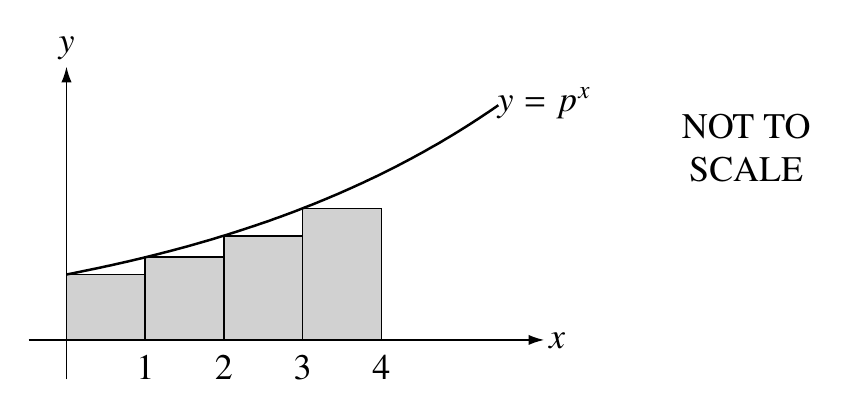
\begin{tikzpicture}[x=0.0127cm,y=-0.0127cm,font=\fontsize{13}{15.6}\selectfont]
\fill[shade] (306.2,329.5) rectangle (385.0,197.9);
\fill[shade] (227.5,329.5) rectangle (306.2,225.2);
\fill[shade] (148.8,329.5) rectangle (227.5,246.8);
\fill[shade] (70.0,329.5) rectangle (148.8,264.0);
\draw (70.0,329.5) rectangle (148.8,264.0);
\draw (148.8,329.5) rectangle (227.5,246.8);
\draw (227.5,329.5) rectangle (306.2,225.2);
\draw (306.2,329.5) rectangle (385.0,197.9);
\draw[->] (32,329.5)--(548,329.5);
\draw[->] (70,369)--(70,56);
\draw[line width=0.9pt] plot[smooth] coordinates {(70.0,264.0) (74.9,263.1) (79.7,262.1) (84.6,261.1) (89.4,260.1) (94.3,259.1) (99.1,258.1) (104.0,257.1) (108.8,256.0) (113.7,255.0) (118.5,253.9) (123.4,252.8) (128.2,251.7) (133.1,250.6) (138.0,249.4) (142.8,248.3) (147.7,247.1) (152.5,245.9) (157.4,244.7) (162.2,243.5) (167.1,242.2) (171.9,241.0) (176.8,239.7) (181.6,238.4) (186.5,237.1) (191.3,235.8) (196.2,234.4) (201.1,233.0) (205.9,231.6) (210.8,230.2) (215.6,228.8) (220.5,227.3) (225.3,225.8) (230.2,224.4) (235.0,222.8) (239.9,221.3) (244.7,219.7) (249.6,218.1) (254.4,216.5) (259.3,214.9) (264.2,213.2) (269.0,211.6) (273.9,209.9) (278.7,208.1) (283.6,206.4) (288.4,204.6) (293.3,202.8) (298.1,201.0) (303.0,199.1) (307.8,197.2) (312.7,195.3) (317.6,193.4) (322.4,191.4) (327.3,189.4) (332.1,187.4) (337.0,185.3) (341.8,183.3) (346.7,181.1) (351.5,179.0) (356.4,176.8) (361.2,174.6) (366.1,172.4) (370.9,170.1) (375.8,167.8) (380.7,165.5) (385.5,163.1) (390.4,160.7) (395.2,158.3) (400.1,155.8) (404.9,153.3) (409.8,150.7) (414.6,148.2) (419.5,145.5) (424.3,142.9) (429.2,140.2) (434.0,137.4) (438.9,134.7) (443.8,131.9) (448.6,129.0) (453.5,126.1) (458.3,123.2) (463.2,120.2) (468.0,117.2) (472.9,114.1) (477.7,111.0) (482.6,107.8) (487.4,104.6) (492.3,101.4) (497.1,98.1) (502.0,94.7)};
\node at (70,38) {$y$};
\node at (560,330) {$x$};
\node at (548,93) {$y=p^{x}$};
\node[align=center] at (750,138) {NOT TO\\SCALE};
\node at (148.8,357) {$1$};
\node at (227.5,357) {$2$};
\node at (306.2,357) {$3$};
\node at (385.0,357) {$4$};\end{tikzpicture}
\end{document}
